After examining the preference-based consumer theory, we have concluded that if a continuously differentiable demand function $x(\mathbf{p},w)$ is generated by rational preferences, this demand function must have
certain properties (see Thm.\ref{thm:properties_walrasian_demand}) and have a symmetric and negative semidefinite substitution matrix $S(\mathbf{p},w)$. In this section, we would examine the reverse:
if a demand function $x(\mathbf{p},w)$ has these properties, can it be rationalized by some preferences?

\subsection{Recover Preferences from Demand Functions}\label{chp2:sec4:ssec1}
The recovering $\succsim$ from $x(\mathbf{p},w)$ will be done in 2 steps:
\begin{enumerate}
    \item[-] \textbf{Step 1}: recover $e(\mathbf{p},u)$ from $x(\mathbf{p},w)$
    \item[-] \textbf{Step 2}: recover $\succsim$ from $e(\mathbf{p},u)$  
\end{enumerate}

\subsubsection*{Recover $e(\mathbf{p},u)$ from $x(\mathbf{p},w)$}
The first step is to recover $e(\mathbf{p},u)$ given a Walrasian demand function $x(\mathbf{p},w)$ that has the assumed properties: satisfies Walras' law, homogeneous of degree 0(see Thm.\ref{thm:properties_walrasian_demand}).
And, demand is assumed to be single-valued.

The recovering of $e(\mathbf{p},u)$ relies on the duality property $h(\mathbf{p},u)=x(\mathbf{p},e(\mathbf{p},u))$ and the proposition $h(\mathbf{p},u)=\nabla_{\mathbf{p}}e(\mathbf{p},u)$, combine these two, get:
$$
    \frac{\partial e(\mathbf{p})}{\partial p_i}=x_i(\mathbf{p},e(\mathbf{p})),\forall i=1,\cdots,L
$$
or, in a familiar form of expression
$$
\nabla_{\mathbf{p}}e(\mathbf{p})=x(\mathbf{p},e(\mathbf{p}))
$$

For this system of differential equations to have a solution, we must have $e(\mathbf{p})$ to be \textbf{twice continuously differentiable}, i.e., $e(\mathbf{p})$'s Hessian matrix is \myhl[blue]{\textbf{symmetric}}. Do the twice differentiation of $e(\mathbf{p})$:
\begin{align*}
    \mathrm{D}^2_{\mathbf{p}}e(\mathbf{p}) &= \mathrm{D}_{\mathbf{p}}x(\mathbf{p},e(\mathbf{p})) +\mathrm{D}_w x(\mathbf{p},e(\mathbf{p}))\cdot x(\mathbf{p},e(\mathbf{p}))^T\\
    & = S(\mathbf{p},e(\mathbf{p}))
\end{align*}
we actually get the Slutsky matrix again. Now we can conclude

\begin{enumerate}
    \item[-] $\nabla_{\mathbf{p}}e(\mathbf{p})=x(\mathbf{p},e(\mathbf{p}))$ has a solution $\Leftrightarrow$ the Slutsky matrix $S(\mathbf{p},w)$ being \textbf{symmetric}
    \begin{enumerate}
        \item[-] $\Rightarrow$: proved by the above equation, which requires the Slutsky matrix be the Hessian matrix of $e(\mathbf{p})$, which aligns with Thm.\ref{thm:prop_hick_pricederive}
        \item[-] $\Leftarrow$: by Frobenius theorem (see \hyperref[sssec:frobenius_theorem]{below} for details), the symmetry of $\nabla_{\mathbf{p}}$ at all points of its domain is equivalent to the existence of a solution 
    \end{enumerate}
    \item[-] the solution $e(\mathbf{p},u)$ has the properties of an expenditure function (Thm.\ref{thm:properties_expenditure_func}) $\Leftrightarrow$ the Slutsky matrix $S(\mathbf{p},w)$ being \textbf{negative semidefinite}
\end{enumerate}

Together, we have
\begin{proposition}{conditions of $S(\mathbf{p},w)$ to recover $e(\mathbf{p},u)$}{slutskycondition_recover}
    $S(\mathbf{p},w)$ being \myhl[blue]{\textbf{symmetric}} and \myhl[blue]{\textbf{negative semidefinite}} is the necessary and sufficient condition to recover $e(\mathbf{p},u)$
\end{proposition}

Prop.\ref{prop:slutskycondition_recover} is always true, and it can be linked to the discussion of WARP in the following way:
\begin{enumerate}
    \item[$L=2$] when there are only 2 goods, the Slutsky matrix is automatically symmetric, hence as long as the demand function $x(p_1,p_2,w)$ satisfies WARP (negative semidefiniteness guaranteed), $e(\mathbf{p},u)$ will be recovered:
    
    \begin{enumerate}
        \item[-] step 1: normalize $p_2=1$, pick an arbitrary price-wealth point $(p_1^0,1,w^0)$ and assign utility value $u^0$ to 
        \item[-] step 2: solve the differential equation 
        $$
        \frac{\mathrm{d}e(p_1)}{\mathrm{p_1}}=x_1(p_1,e(p_1))
        $$
        where $e(p_1)=e(p_1,1,u^0)$, $x_1(p_1,w)=x_1(p_1,1,w)$, with the initial condition $e(p_1^0)=w^0$
    \end{enumerate}
    Fig.\ref{fig:recover_exp_from_wal} illustrates the essence of this procedure intuitively: for any $(p_1,w)$, the demand function at the point $x_1(p_1,w)$ is the slope of some expenditure function, and for any given initial condition $(p_1^0,w^0)$, there will be an expenditure curve starts at it.
    \item[$L>2$] when there are more than 2 goods, WARP does not guarantee the symmetry of the Slutsky matrix, hence, symmetry condition must also be satisfied for the recovery of $e(\mathbf{p},u)$
\end{enumerate} 

\begin{figure}[ht]
    \centering
    \caption{Recover $e(\mathbf{p},u)$ from $x(\mathbf{p},w)$}
    \label{fig:recover_exp_from_wal}
    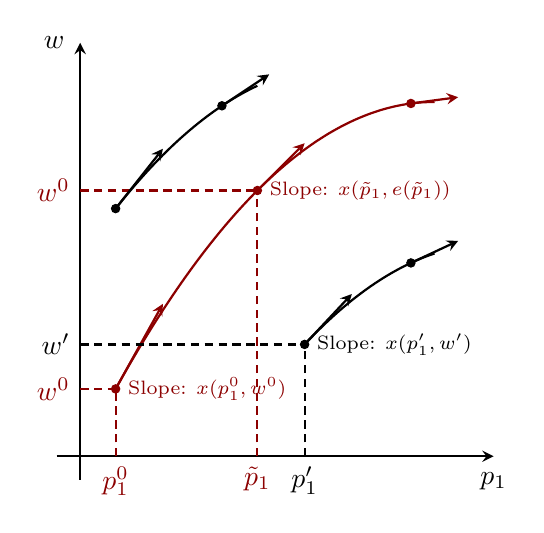
\begin{tikzpicture}[scale=1.5]
        % basics
        \draw [-stealth,color=black,thick] (-0.2,0) -- (3.5,0) node[below=2pt] {$p_1$};
        \draw [-stealth,color=black,thick] (0,-0.2) -- (0,3.5) node[left=2pt] {$w$};
        
        % correct e(p,u)
        \draw[domain=0.3:3, smooth, thick, red!55!black, variable=\x] plot ({\x}, {-1/3*(\x-3)^2+3});
        %% tangent 1
        \draw [-stealth,color=red!55!black,thick] (0.3,0.57) -- (0.7,1.29);
        \filldraw[red!55!black] (0.3,0.57) circle (1pt) node[right=1pt] {\scriptsize Slope: $x(p_1^0,w^0)$}; % initial bundle
        \draw[densely dashed,thick,red!55!black] (0.3,0) node[below] {$p_1^0$} --  (0.3,0.57);
        \draw[densely dashed,thick,red!55!black] (0,0.57) node[left] {$w^0$} -- (0.3,0.57);
        %% tangent 2
        \draw [-stealth,color=red!55!black,thick] (1.5,2.25) -- (1.9,2.65);
        \filldraw[red!55!black] (1.5,2.25) circle (1pt) node[right=1pt] {\scriptsize Slope: $x(\tilde{p}_1,e(\tilde{p}_1))$};
        \draw[densely dashed,thick,red!55!black] (1.5,0)  node[below] {$\tilde{p}_1$} -- (1.5,2.25);
        \draw[densely dashed,thick,red!55!black] (0,2.25) node[left] {$w^0$} -- (1.5,2.25);
        %% tangent 3
        \draw [-stealth,color=red!55!black,thick] (2.8,2.9867) -- (3.2,3.04);
        \filldraw[red!55!black] (2.8,2.9867) circle (1pt);
        
        % alternate 1
        \draw[domain=1.9:3, smooth, thick, black, variable=\x] plot ({\x}, {-1/3*(\x-3.5)^2+1.8});
        %% tangent a1
        \draw [-stealth,color=black,thick] (1.9,0.9467) -- (2.3,1.37337);
        \filldraw[black] (1.9,0.9467) circle (1pt) node[right=1pt] {\scriptsize Slope: $x(p'_1,w')$}; % initial bundle
        \draw[densely dashed,thick,black] (1.9,0) node[below] {$p'_1$} --  (1.9,0.9467);
        \draw[densely dashed,thick,black] (0,0.9467) node[left] {$w'$} -- (1.9,0.9467);
        %% tangent a2
        \draw [-stealth,color=black,thick] (2.8,1.6367) -- (3.2,1.82337);
        \filldraw[black] (2.8,1.6367) circle (1pt);
        
        % alternate 2
        \draw[domain=0.3:1.5, smooth, thick, black, variable=\x] plot ({\x}, {-1/3*(\x-2.2)^2+3.3});
        %% tangent b1
        \draw [-stealth,color=black,thick] (0.3,2.0967) -- (0.7,2.6033);
        \filldraw[black] (0.3,2.0967) circle (1pt);
        %% tangent b2
        \draw [-stealth,color=black,thick] (1.2,2.967) -- (1.6,3.233);
        \filldraw[black] (1.2,2.967) circle (1pt);
        
    \end{tikzpicture}
\end{figure}

\subsubsection*{Recover $\succsim$ from $e(\mathbf{p},u)$}
The second step is to recover $\succsim$ given an expenditure function $e(\mathbf{p},u)$ that has the assumed properties: continuous, strictly increasing in $u$, non-decreasing, homogeneous of degree 1, and concave in $\mathbf{p}$ (see Thm.\ref{thm:properties_expenditure_func}).
Since demand is single-valued, $e(\mathbf{p},u)$ is also differentiable.

Here, let $V_u\subset \mathbb{R}^L$  be an at-least-as-good-as set for each utility level $u$ s.t. $e(\mathbf{p},u)$ is the minimal expenditure required for a bundle in $V_u$ at price $\mathbf{p}\gg  0$, i.e. 
$$
e(\mathbf{p},u)=\min_{\mathbf{x}\geq 0}\mathbf{p}\cdot \mathbf{x}\ \text{ s.t. }\mathbf{x}\in V_u
$$

Intuitively, the set $V_u = \left\{ \mathbf{x} \in\mathbb{R}^L_+\mid \mathbf{p}\cdot \mathbf{x}\geq e(\mathbf{p},u),\forall \mathbf{p}\gg 0 \right\}$ satisfies the requirement, that is 
\begin{proposition}{At-least-as-good-as set $V_u$}{atleastasgoodasset_exp}
    For $e(\mathbf{p},u)$ that is strictly increasing in $u$, continuous, non-decreasing, homogeneous of degree 1, concave and differentiable in $\mathbf{p}$, then $\forall u$, $e(\mathbf{p},u)$ is the expenditure function associated with the at-least-as-good-as set
    $$
    V_u = \left\{ \mathbf{x}\in\mathbb{R}^L_+\mid \mathbf{p}\cdot\mathbf{x}\geq e(\mathbf{p},u),\forall \mathbf{p}\gg 0 \right\}
    $$
    i.e. $e(\mathbf{p},u)=\min\left\{ \mathbf{p}\cdot \mathbf{x}\mid \mathbf{x}\in V_u \right\},\forall \mathbf{p}\gg 0$.
\end{proposition}

\textbf{Proof}: Immediately by definitions, $e(\mathbf{p},u)\leq \min\left\{\mathbf{p}\cdot\mathbf{x}\mid \mathbf{x}\in V_n\right\}$. Next, prove $e(\mathbf{p},u)\geq \min\left\{\mathbf{p}\cdot\mathbf{x}\mid \mathbf{x}\in V_n\right\}$: since $e(\mathbf{p},u)$ is concave in $\mathbf{p}$, we have
$$
e(\mathbf{p}',u)\leq e(\mathbf{p},u)+\nabla_{\mathbf{p}}e(\mathbf{p},u)\cdot(\mathbf{p}'-\mathbf{p}),\forall \mathbf{p},\mathbf{p}'
$$
since $e(\mathbf{p},u)$ is homogeneous of degree 1, by Euler's formula, $e(\mathbf{p},u)=\mathbf{p}\cdot\nabla_{\mathbf{p}}e(\mathbf{p},u)$, hence $e(\mathbf{p}',u)\leq \mathbf{p}'\cdot \nabla_{\mathbf{p}}e(\mathbf{p},u),\forall \mathbf{p}'$, plus the fact that $\nabla_{\mathbf{p}(\mathbf{p},u)}\geq 0$, gives that $\nabla_{\mathbf{p}(\mathbf{p},u)}\in V_u$.
By the definition of the at-least-as-good-as set $V_u$, we have $\min\left\{\mathbf{p}\cdot\mathbf{x}\mid \mathbf{x}\in V_u\right\}\leq \mathbf{p}\cdot \nabla_{\mathbf{p}(\mathbf{p},u)}=e(\mathbf{p},u)$. The proof is finished.

With Prop.\ref{prop:atleastasgoodasset_exp}, we can find a set of $V_u$ for each level of $u$, and since $\partial e(\mathbf{p},u)/\partial u>0$, we have $u'>u\Rightarrow V_{u'}\subset V_u$. Each $V_u$ is closed, convex, and bounded below, hence these at-least-as-good-as sets can define a 
preference $\succsim$ (represented by utility levels $u$) that has $e(\mathbf{p},u)$ as its expenditure function (see Fig.\ref{fig:recover_pref_from_exp}).

\begin{figure}[ht]
    \centering
    \caption{Recover $\succsim$ from $e(\mathbf{p},u)$}
    \label{fig:recover_pref_from_exp}
    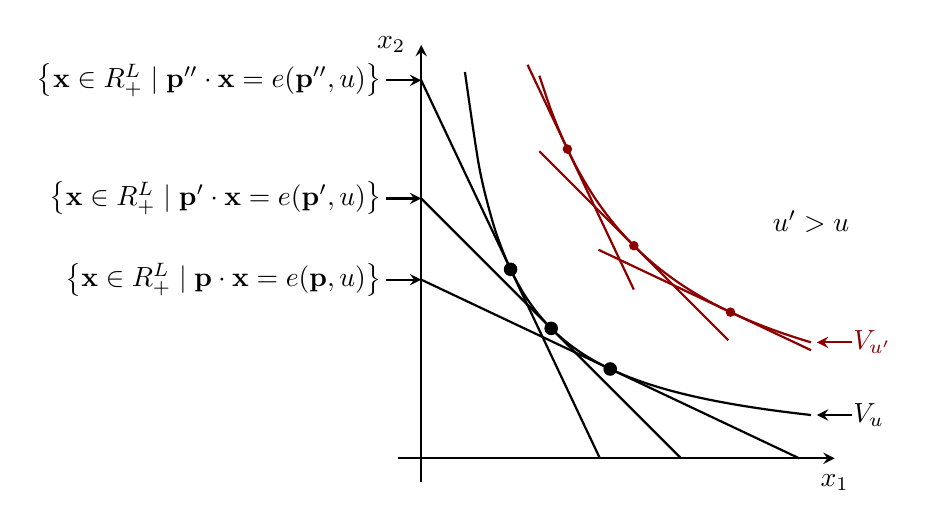
\begin{tikzpicture}[scale=1.5]
        % basics
        \draw [-stealth,color=black,thick] (-0.2,0) -- (3.5,0) node[below=2pt] {$x_1$};
        \draw [-stealth,color=black,thick] (0,-0.2) -- (0,3.5) node[left=2pt] {$x_2$};
        
        % utility and budget lines
        \draw[domain=0.37:3.3, smooth, thick, black, variable=\x] plot ({\x}, {1.1^2/\x}); % utility
        
        \draw[domain=1:3.3, smooth, thick, red!55!black, variable=\x] plot ({\x}, {1.8^2/\x}); % utility'
        
        \draw[domain=0:(4*1.1^2)/3.2, black, thick, variable=\x] plot ({\x}, {3.2-(3.2^2/(4*1.1^2))*\x}); % budget 1
        \draw[domain=0:2.2,black, thick, variable=\x] plot ({\x}, {2.2-\x}); % budget 2
        \draw[domain=0:3.2, black, thick, variable=\x] plot ({\x}, {((4*1.1^2)/3.2)-((4*1.1^2)/3.2^2)*\x}); % budget 3
        
        \draw[domain=0.9:1.8, red!55!black, thick, variable=\x] plot ({\x}, {5.23636-(3.2^2/(4*1.1^2))*\x}); % budget 1'
        \draw[domain=1:2.6,red!55!black, thick, variable=\x] plot ({\x}, {3.6-\x}); % budget 2'
        \draw[domain=1.5:3.3, red!55!black, thick, variable=\x] plot ({\x}, {2.475-((4*1.1^2)/3.2^2)*\x}); % budget 3'
        
        
        
        % bundles
        \filldraw[black] (0.75625,1.1^2/0.75625) circle (1.5pt); % bundle 1
        \filldraw[black] (1.1,1.1) circle (1.5pt); %  bundle 2
        \filldraw[black] (1.1^2/0.75625,0.75625) circle (1.5pt); % bundle 3
         % bundles
        \filldraw[red!55!black] (1.2375,1.8^2/1.2375) circle (1pt); % bundle 1'
        \filldraw[red!55!black] (1.8,1.8) circle (1pt); %  bundle 2'
        \filldraw[red!55!black] (1.8^2/1.2375,1.2375) circle (1pt); % bundle 3'
        
        %% utility
        \draw[stealth-,thick] (3.35,1.1^2/3.3) -- node[right=3pt] {$V_u$} (3.65,1.1^2/3.3);
        \draw[stealth-,thick,red!55!black] (3.35,1.8^2/3.3) -- node[right=3pt] {$V_{u'}$} (3.65,1.8^2/3.3);
        
        % texts and notes
        %% budget change
        \draw[-stealth,thick,black] (-0.3,3.2) -- node[left=4pt] {$\left\{\mathbf{x}\in\mathbb{R}^L_+\mid \mathbf{p}''\cdot\mathbf{x}=e(\mathbf{p}'',u) \right\}$} (0,3.2);
        \draw[-stealth,thick,black] (-0.3,2.2) -- node[left=4pt] {$\left\{\mathbf{x}\in\mathbb{R}^L_+\mid \mathbf{p}'\cdot\mathbf{x}=e(\mathbf{p}',u) \right\}$} (0,2.2);
        \draw[-stealth,thick,black] (-0.3,1.5125) -- node[left=4pt] {$\left\{\mathbf{x}\in\mathbb{R}^L_+\mid \mathbf{p}\cdot\mathbf{x}=e(\mathbf{p},u) \right\}$} (0,1.5125);
        
        \node at (3.3,2) {$u'>u$};
        
    \end{tikzpicture}
\end{figure}

This conclusion can be extended to the case that the underlying preferences of $e(\mathbf{p},u)$ is \textbf{non-convex}. A non-convex $\succsim$ will generate a non-convex 
at-least-as-good-as set, as shown in Fig.\ref{fig:recover_pref_from_exp_nonconvex}.

\begin{figure}[ht]
    \centering
    \caption{Recover non-convex $\succsim$ from $e(\mathbf{p},u)$}
    \label{fig:recover_pref_from_exp_nonconvex}
    \begin{tikzpicture}[scale=1.5]
        % basics
        \draw [-stealth,color=black,thick] (-0.2,0) -- (3.5,0) node[below=2pt] {$x_1$};
        \draw [-stealth,color=black,thick] (0,-0.2) -- (0,3.5) node[left=2pt] {$x_2$};
        
        \draw [thick,red!55!black,tangent=0.9] (0.37,3.3) .. controls (0.5,2.2) and (0.6,1.5) .. (0.8,1.5);
        \draw [black, thick, use tangent] (-1,0) -- (2,0);
        
        \draw [thick,red!55!black,tangent=0.1] (1.5,0.8) .. controls (1.5,0.6) and (2.2,0.5) .. (3.3,0.37);
        \draw [black, thick, use tangent] (-2,0) -- (1,0);
        
        %non-convex part
        \draw [thick,dashed,red!55!black] (0.8,1.5).. controls (1.4,1.4).. (1.5,0.8);
        \draw[domain=0.2:2.05,red!55!black, thick, variable=\x] plot ({\x}, {2.25-\x});
        
        % notes
        %%% actual
        \draw[stealth-,dashed, thick,red!55!black] (1.36,1.36) -- node[right=5pt,yshift=10pt,align=left] {Boundary of \textbf{actual} \\ at-least-as-good-as set} (1.7,1.7);
         %%% Slutsky
        \draw[-stealth,thick,black] (1.125-0.4,1.125-0.4) -- node[left=5pt,yshift=-10pt] {Boundary of $V_u$} (1.12,1.12);
        %%% price-utility
        \draw[stealth-,thick,black] (2.05,0.2) -- node[right=5pt] {\scriptsize $\left\{\mathbf{x}\in\mathbb{R}^L_+\mid \mathbf{p}^*\cdot\mathbf{x}=e(\mathbf{p}^*,u^*)\right\}$} (2.4,0.2);
    \end{tikzpicture}
\end{figure}

For this non-convex at-least-as-good-as set, we can always find its convex hull (the solid line) that also generates the
expenditure function $e(\mathbf{p}),u)$. 
Here we have the correspondence between the differentiability of $e(\mathbf{p},u)$ and the , for a specific price-utility pair $(\mathbf{p}^*,u^*)$, there would be more than one expenditure minimizers, and at this price-utility pair $(\mathbf{p}^*,u^*)$,
 the generated $e(\mathbf{p},u)$ would \textbf{NOT} be differentiable. This can be summarized as:
$$
e(\mathbf{p},u) \text{ is differentiable}\Rightarrow \succsim \text{ is convex}
$$

With the two steps, $\succsim$ can be recovered from demand function $x(\mathbf{p},w)$ through expenditure function $e(\mathbf{p},u)$. This problem, especially the problem of recovering $e(\mathbf{p},u)$ from $x(\mathbf{p},u)$, which involves the differential equation $h(\mathbf{p},u)=\nabla_{\mathbf{p}}e(\mathbf{p},u)$, is the \textbf{integrability} problem.

\subsection{Discussion on integrability}\label{sssec:integrability}
The discussion on recovering preferences from demand functions is based on Hurwicz and Uzawa's work, to summarize, we have
\begin{enumerate}
    \item[-] \myhl[blue!45!black]{\textbf{(B)}}: \underline{\textbf{budget}} exhaustion: $\mathbf{p}\cdot x(\mathbf{p},w)=w$
    \item[-] \myhl[blue!45!black]{\textbf{(D)}}: the demand function $x(\mathbf{p},w)$ is \underline{\textbf{differentiable}} everywhere
    \item[-] \myhl[blue!45!black]{\textbf{(S)}}: the Slutsky matrix $S(\mathbf{p},w)$ is \underline{\textbf{symmetric}}
    \item[-] \myhl[blue!45!black]{\textbf{(NSD)}}: the Slutsky matrix $S(\mathbf{p},w)$ is \underline{\textbf{negative semidefinite}}
    \item[-] \myhl[blue!45!black]{\textbf{(IB)}}: the demand function $x(\mathbf{p},w)$ satisfies the \underline{\textbf{boundedness}} condition: $$ \left\vert \frac{\partial x_i(\mathbf{p},w)}{\partial w} \right\vert \leq M < \infty, \forall i=1,\cdots,n,\forall m\geq 0 $$
\end{enumerate}

These assumptions are required for the process of recovering preferences from demand functions discussed above: If all 5 of Hurwicz-Uzawa assumptions are satisfied, then $\exists u$ s.t. $\forall (\mathbf{p},w)$, $x(\mathbf{p},w)$ is the \myhl[blue!45!black]{\textbf{unique}} maximizer of $u$ over the budget set $\left\{ \mathbf{x}: \mathbf{p}\cdot \mathbf{x}\leq w\right\}$.

To integrate from demand $x(\mathbf{p},w)$ to a utility function, it is sufficient to integrate from $x(\mathbf{p},w)$ to the indirect utility function $v(\mathbf{p},w)$, then $x(\cdot)$ and $v(\cdot)$ must satisfy the Hotelling's lemma:
$$
-\frac{v_{\mathbf{p}}(\mathbf{p},w)}{v_{w}(\mathbf{p},w)} = \mathbf{x}(\mathbf{p},w)
$$
From this, we have two separate aspects to understand integrability: 
\begin{enumerate}
    \item[-] \textit{mathematical} integrability: the existence of $v(\cdot)$ to satisfy the differential equation above.
    \item[-] \textit{economic} integrability: $v(\cdot)$ should be a well-behaved indirect utility function as well, corresponding to a direct utility function.
\end{enumerate}

This result is quite general and is one of the fundamental results, some recent work seeks to extend it to reflect the nuance of empirical observations. I have searched some papers on this topic and will briefly discussed the results here. For a rather thorough discussion on the development of this topic, see \citet*{hands2006integrability}.

\subsubsection*{Incomplete systems of demand functions}
Hurwicz and Uzawa's result is theoretically exhaustive, in the sense that as long as the 5 integrability conditions are satisfied, with suitable regularity conditions assumed, \textbf{any} set of demand functions can be retionalized by some utility function. \cite{epstein1982integrability} discussed the problem of incomplete sets of demand functions.

Consider the utility maximization problem of a consumer:
$$
\max_{\mathbf{x},\mathbf{y},z} \left\{ u(\mathbf{x},\mathbf{y},z)\mid \mathbf{p}\cdot\mathbf{x}+\mathbf{q}\cdot \mathbf{y} + z =w, \mathbf{x},\mathbf{y},z\geq 0 \right\}
$$
where $\mathbf{x}$ is the set of \textbf{observed} demands (priced at $\mathbf{p}$), and $\left(\mathbf{y},z\right)$ is the unobservable set of demands (priced as $(\mathbf{q},1)$, z is the numeraire). If the observed $\mathbf{x}$ is part of the solution to the utility maximization problem, it will have some of the properties (notably symmetry and negative semi-definiteness) like that for complete demand systems. However, Hurwicz-Uzawa integrability conditions are \textbf{not enough} to guarantee the
existence of a utility function for incomplete demand functions. Instead, they proposed that if the observed demand function $\mathbf{x}(w,\mathbf{p},\mathbf{q}): \Omega^{1+n+m}\rightarrow \Omega^n$\sidenotes{$\leftarrow$ $n$ observed, $m+1$ unobserved} such that 
\begin{enumerate}
    \item[1.] budget binding: $\forall (w,\mathbf{p},\mathbf{q})$, $\mathbf{p}x(w,\mathbf{p},\mathbf{q})<w,x(w,\mathbf{p},\mathbf{q})>0$
    \item[2.] $x^i(w,\mathbf{p},\mathbf{q})$ is \textbf{twice continuously differentiable} for all $i$
    \item[3.] The $n\times n$ matrix $x_{\mathbf{p}}(w,\mathbf{p},\mathbf{q}) + x(w,\mathbf{p},\mathbf{q})\cdot x_w (w,\mathbf{p},\mathbf{q})$ (Slutsky matrix for observed demands) is \textbf{negative \myhl[red!55!black]{definite}}
\end{enumerate}
Then there exists a \textbf{continuous, non-decreasing and \myhl[red!55!black]{quasiconcave}} utility function $u$ and a \myhl[red!55!black]{\textbf{neighborhood}} $N$ of $(w^0,\mathbf{p}^0,\mathbf{q}^0)$ s.t. $\forall (w,\mathbf{p},\mathbf{q})\in N$, $x(w,\mathbf{p},\mathbf{q})$ is the unique solver of the aforementioned utility maximizing problem.

The key argument of \cite{epstein1982integrability} is the \textbf{negative \myhl[red!55!black]{definiteness}} of the Slutsky matrix of the observed demands, and one thing very important about this result is that it is a \myhl[red!55!black]{\textbf{local}} result. The proof is skipped here, but duality also plays a crucial role as before.

To extend this local result to possible global results, some extra conditions must be met. \citet*{epstein1982integrability} proposed that if $x_{\mathbf{q}}(w,\mathbf{p},\mathbf{q})=0$, the 3 conditions will guarantee the glocal integrability of $x(\cdot)$, that is, observed demands (the first $n$ goods) are independent of the prices of the remaining $(m+1)$ goods (demands unobserved). This result is quite intuitive: consider the case of $n=1$, that is, the demand of only one good is observed. If other (normalized) prices $\mathbf{q}$ are constant, then this problem can fit into a two-good framework and the standard integrability results apply. \citet*{epstein1982integrability} also proposed several classes of demand functions $x(\cdot)$ that have global integrability (see Table 1 on Page 419 of the paper for details).

\citet*{lafrance1989dual} generalized \citeauthor*{epstein1982integrability}'s result by employing an arbitrary price index for the goods of which the demand is unobserved: $\pi(\mathbf{q})$. This deflator function $\pi(\mathbf{q})$\footnote{some examples are: $\pi(\mathbf{q})\equiv q_1$, $\pi(\mathbf{q})\equiv \sum^m_{j=1}\alpha_jq_j$, $\pi(\mathbf{q})\equiv \prod^m_{j=1}q_j^{\alpha_j}$, where $\sum^m_{j=1}\alpha_j=1,\alpha_j\geq 0$.} is used to normalize $\mathbf{p}$ and $w$. In addition to the 3 conditions of \citeauthor*{epstein1982integrability}, \citeauthor*{lafrance1989dual} gave a condition on $\pi(\mathbf{q})$ to guarantee the \myhl[blue!45!black]{\textbf{global}} integrability: $\exists \pi:\mathbb{R}^m_{++}\rightarrow \mathbb{R}_+$ s.t. $\pi\in C^2$ is \textbf{increasing}, \textbf{homogeneous of degree 1}, \textbf{concave in }$\mathbf{q}$ and $x(w,\mathbf{p},\mathbf{q})=\tilde{x}\left(\frac{1}{\pi(\mathbf{q})}\cdot w,\frac{1}{\pi(\mathbf{q})}\cdot\mathbf{p}\right)$. This condition requires that the observed demands depend upon the prices of other goods \textbf{only} through a price index that deflates the prices of the observed goods and total expenditure. 

However, this condition depends on the separability of $\mathbf{q}$ from $(\mathbf{p},w)$ in the indirect utility function: $v(w,\mathbf{p},\mathbf{q})\equiv \varphi\left(\frac{w}{\pi(\mathbf{q})},\frac{w}{\pi(\mathbf{q})}\right)$ and in the expediture function $e(u,\mathbf{p},\mathbf{q})\equiv \pi(\mathbf{q})\epsilon\left(\frac{\mathbf{p}}{\pi(\mathbf{q})},u\right)$. This is equivalent to a homothetically separable utility function: $u(\mathbf{x},\mathbf{y})\equiv \bar{u}\left(\mathbf{x},f(\mathbf{y})\right)$\sidenotes{$\leftarrow$ here the notation is modified for convenience, $\mathbf{x}$ is still the vector of observed demands, $\mathbf{y}$ is the vector of unobserved demands}, where $f(\cdot)$ is homogeneous of degree 1. Obviously, this is a very restrictive condition. Therefore, \citeauthor*{lafrance1989dual} introduced the concept of \myhl[red!55!black]{\textbf{weak integrability}}: If $\forall (w,\mathbf{p},\mathbf{q})$, there is a function $\nu:\mathbb{R}^{n+m+1}_{++}\rightarrow \mathbb{R}$ that is \textbf{continuous, increasing and quasiconcave} in $(\mathbf{x},s)$ where $\mathbf{x} = x(w,\mathbf{p},\mathbf{q})$ and $s=\sigma(w,\mathbf{p},\mathbf{q})\equiv y-\mathbf{p}\cdot\mathbf{x}$\footnote{Here, $\mathbf{x}$ is still the observed demands, and $s$ is the expenditure on all other goods: $s\equiv \mathbf{q}\cdot \mathbf{z}$} solves the maximization problem:
$$
\max_{\mathbf{x},s}\left\{ \nu(\mathbf{x},s,\mathbf{q}) \mid \mathbf{p}\cdot\mathbf{x}+s\leq w, \mathbf{x}\geq 0,s>0 \right\}
$$
and the duality is established in the same way as the complete demand system: \textbf{weak} integrability is equivalent to the existence of an expenditure function $e(\mathbf{p},\mathbf{q},u)$ that is increasing and concave in $\mathbf{p}$, homogeneous of degree 1 in $(\mathbf{p},\mathbf{q})$, and satisfies 
$$
\mathbf{p}\cdot x(e(\mathbf{p},\mathbf{q},u),\mathbf{p},\mathbf{q}) + \sigma(e(\mathbf{p},\mathbf{q},w),\mathbf{p},\mathbf{q})\equiv e(\mathbf{p},\mathbf{q},u)
$$
and Hotelling's lemma. 

\citeauthor*{lafrance1989dual} proved that the following conditions need to be satisfied to achieve (global) weak integrability:
\begin{enumerate}
    \item[-] $x(\cdot)\in C^2$, homogeneous of degree 0 in $(w,\mathbf{p},\mathbf{q})$
    \item[-] $x(w,\mathbf{p},\mathbf{q})\geq 0$, $\mathbf{p}\cdot x(w,\mathbf{p},\mathbf{q})<w$ (positive and not budget-exhausting)
    \item[-] Slutsky matrix $S$ is \textbf{symmetric, negative \myhl[red!55!black]{semidefinite}}
\end{enumerate} 
These conditions are pretty much the same as the integrability condition for complete demand systems. In addition,
\begin{enumerate}
    \item[-] $e(\cdot)\in C^3$ in $\mathbf{p}$: extra degree of differentiability to guarantee $x(\cdot)\in C^2$
    \item[-] $\forall (w,\mathbf{p},\mathbf{q})$, $s$ satisfies $\frac{\partial s_{ij}}{\partial w}=\frac{\partial s_{ji}}{\partial w}$ and $\frac{\partial s_{ij}}{\partial p_k}=\frac{\partial s_{ji}}{\partial p_k},\forall i,j,k=1,\cdots, n$: given by the symmetry of Slutsky matrix.
\end{enumerate}
These conditions are much easier to satisfy and verify empircally. \citeauthor*{lafrance1989dual} also discussed welfare implications of this result.

\subsubsection*{Linear and quasi-linear integrability}

\citet*{amir2017microeconomic} surveys the microfoundation of \textbf{linear demand} and discussed the integrability of it. Linear demand is the solution to the quadratic utility maximization problem, 

Consider the numeraire as additively separable, the UMP is then:
\begin{align*}
    \max & U(\mathbf{x})+y & \text{s.t. }&\mathbf{p}\cdot\mathbf{x}+y\leq w
\end{align*}
with Walrasian demand $(\mathbf{x}^*,y^*)$ as its solution. 

Its dual problem (EMP) is 
\begin{align*}
    \min & \mathbf{p}\cdot\mathbf{x}+y & \text{s.t. }U(\mathbf{x})+y&\geq u
\end{align*}
with Hicksian demand $(\mathbf{x}^h,y^h)$ as its solution.
\citeauthor*{amir2017microeconomic} showed that under quasi-linear utility, both the Walrasian demand and the Hicksian demand satisfy the Law of Demand\footnote{For the Hicksian demand: by convex analysis, $\frac{\partial e(\mathbf{p},u)}{\partial p_i}=x^h_i$ (which is just Shepard's Lemma). For Walrasian, since utility is quasi-linear in the numeraire, there are no income effects.}. Here, the result does NOT reply on the classic assumption that the utility function is quasi-concave.

Now we look at the case of quadratic utility: $U(x)=\mathbf{a}'\mathbf{x}-\frac{1}{2}\mathbf{x}'\mathbf{B}\mathbf{x}$, where $\mathbf{a}\in \mathbb{R}^n_{++}$, $\mathbf{B}$ is an $n\times n$ matrix, normalized to be symmetric and have all its diagonal entries equal to 1. Then the utility maximization problem is
$$
\max \left\{ \mathbf{a}'\mathbf{x}-\frac{1}{2}\mathbf{x}'\mathbf{B}\mathbf{x}+y \right\}\ \text{s.t. }\mathbf{p}'\mathbf{x}+y=w
$$
Here, the demand function is linear \sidenotes{The demand function is actually an \textbf{affine} function whenever positive and 0 otherwise, to be precise.}, for the consumer's problem to have an \myhl[blue!45!black]{\textbf{interior}} solution and preserve the \myhl[blue!45!black]{\textbf{linear}} nature of the resulting demand function, we need:
\begin{align*}
    \mathbf{B}^{-1}(\mathbf{a}-\mathbf{p})&>0 & \mathbf{p}'\mathbf{B}^{-1}(\mathbf{a}-\mathbf{p})\leq w
\end{align*}
so the essential condition here is $\mathbf{B}$ is \myhl[red!55!black]{\textbf{inversible}}, i.e., $U$ is \textbf{strictly} concave. This gives a significant result: $\mathbf{B}$ is positive definite, then the inverse demand and the direct demand satisfy the \myhl[blue!45!black]{\textbf{strict Law of Demand}}:
$$
\left[ U(\mathbf{x}) - U(\mathbf{x}') \right]\cdot \left( \mathbf{x}-\mathbf{x}' \right) <0,\ \forall \mathbf{x},\mathbf{x}'\in \mathbb{R}^n_{+}
$$
let $\mathbf{M}=\mathbf{B}^{-1}$, then $\exists$ a continuous utility $U:\mathbb{R}^n_{+}\rightarrow \mathbb{R}$ s.t. the linear demand function $D(\mathbf{p})=\mathbf{d}-\mathbf{Mp}$ with $d_i\geq 0,\forall i$ can be obtained by solving
$$
\max\left\{U(\mathbf{x}+y)\right\}\ \text{s.t.}\mathbf{p'x}+y\leq w
$$
since $\mathbf{M}=\mathbf{B}^{-1}$, it is symmetric and positive definite as well.
Using this result, \citeauthor*{amir2017microeconomic} discussed a widely used utility specification characterized by a \textbf{fully symmetric} substitution/complementarity matrix
$$
\mathbf{B}=\begin{bmatrix}
    1 & \gamma &\cdots &\gamma\\
    \gamma & 1 & \ddots & \vdots\\
    \vdots & \ddots & \ddots & \gamma\\
    \gamma & \cdots & \gamma & 1
\end{bmatrix}
$$
for it to be strictly concave, $\gamma\in \left(-\frac{1}{n-1},1\right)$. 
The main message of this result is that any linear demand that maximizes the utility of a representative consumer necessarily possesses strong regularity properties.

\citet*{nocke2017quasi} extended the quasi-linear integrability for all continuous demand systems that do not depend on income, their approach is:
\begin{enumerate}
    \item[1.] show the existense of an indirect subutility function
    \item[2.] construct a direct quasi-linear utility function with duality theory
    \item[3.] show that: quasi-linear integrability $\Leftrightarrow$ the demand system being a \myhl[red!55!black]{\textbf{conservative}} vector field $\Leftrightarrow$  \myhl[red!55!black]{\textbf{symmetric}} and \myhl[red!55!black]{\textbf{negative semidefinite}} substitution matrix\sidenotes{$\leftarrow$\textbf{NO} income here, demand system is assumed to be independent of income}
\end{enumerate}

The main result is 3, that is, for a \textbf{continuous} demand $D(\cdot)\in C^1$, the following are equivalent:
\begin{enumerate}
    \item[(a)] $D$ is quasi-linearly integrable: $\exists \mathbf{X}\subseteq \mathbb{R}^n_+$ and $u(\cdot):\mathbf{X}\rightarrow \mathbb{R}$ s.t. $\forall (p_0,\mathbf{p},w)\in\mathbb{R}_{++}\times \mathbb{R}^n_{++}\times \mathbb{R}_+$, $D(p_0,\mathbf{p},w)$ is the unique solution of 
    $$\max_{x_0,\mathbf{x}}x_0+u(\mathbf{x}) \text{ s.t. } p_0x_0+\mathbf{p}\cdot\mathbf{x}\leq w, x_0\geq 0,\mathbf{x}\in \mathbf{X}
    $$
    \item[(b)] $\forall k\geq 2$ and $\mathbf{p}^{i\in \{1\cdots k\}}\in \left(\mathbb{R}^n_{++}\right)^k$, $$ \left(\mathbf{p}^2-\mathbf{p}^1\right)\cdot D\left(\mathbf{p}^1\right) +\cdots \left(\mathbf{p}^k-\mathbf{p}^{k-1}\right)\cdot + D\left(\mathbf{p}^{k-1}\right) + \left(\mathbf{p}^1-\mathbf{p}^k\right)\cdot D\left(\mathbf{p}^k\right)\geq 0 $$
    \item[(c)] $D(\cdot)$ is conservative $$ \int_C D(\mathbf{p})\mathrm{d}\mathbf{p}=0,\ \forall C$$ where $C$ is a closed and piecewise-continuously differentiable path\footnote{A closed and piecewise-continuously differentiable path is a continuous function $p:[0,1]\rightarrow \mathbb{R}^n_{++}$ s.t. $p$ is piecewise $C^1$ and $p(0)=p(1)$, the line integral $\int_C D(p)\mathrm{d}p=\int^1_0 p'(t)D(p(t))\mathrm{d}t$}; and satisfies the law of demand $$ (\mathbf{p}'-\mathbf{p})\cdot (D(\mathbf{p}')-D(\mathbf{p}))\leq 0, \ \forall \mathbf{p},\mathbf{p}' $$
    \item[(d)] $\forall \mathbf{p}\gg 0$, the substitution matrix $J(\mathbf{p})\equiv \left(\frac{\partial D_i}{\partial p_i}(\mathbf{p})\right)_{1\leq i,j\leq n}$ is \textbf{symmetric} and \textbf{negative semi-definite}.
\end{enumerate}

The detailed proof of this result is presented in their paper, but the intuition is:
\begin{enumerate}
    \item[-] \underline{\textit{Step 1}}: If $D$ can be indirectly derived from $v$, then $\nabla v=-D$, and if $D(\cdot)$ satisfies (c), $\exists v$ s.t. $\nabla v=-D$
    \item[-] \underline{\textit{Step 2}}: prove that (a) $\Rightarrow$ (b), relying on \textit{Step 1}, specifically, the convexity of $v$
    \item[-] \underline{\textit{Step 3}}: construct $(\mathbf{X},u)$ as:
    \begin{enumerate}
        \item[-] $u(\mathbf{x})=\inf_{\mathbf{p}\gg 0}\left\{\mathbf{p}\cdot\mathbf{x}+v(\mathbf{p})\right\}$ satisfies
        \begin{enumerate}
            \item[$\cdot$] quasilinearity: $\forall \mathbf{p}\gg 0, u(D(\mathbf{p}))=\mathbf{p}\cdot D(\mathbf{p})+v(\mathbf{p})$
            \item[$\cdot$] concavity and monotonicity (non-decreasing) 
        \end{enumerate}
        \item[-] $\mathbf{X}=\left\{ \mathbf{x} \in \mathbb{R}^n_+\mid u(\mathbf{x}) \text{ is finite} \right\}$ satisfies
        \begin{enumerate}
            \item[$\cdot$] The comprehensive convex hull\footnote{The comprehensive convex hull (CCH) of $X$ is the smallest set that contains $X$ that is \textbf{convex} and \textbf{comprehensive upward}.} of $\mathcal{R}(D)$ is a subset of $\mathbf{X}$, where $\mathcal{R}(D)$ denotes the range of $D$.
        \end{enumerate}
    \end{enumerate}
    \item[-] \underline{\textit{Step 4}}: show that $D$ can be derived from $(\mathbf{X},u)$, that is $\forall (p_0,\mathbf{p},w)\geq 0$, $\forall (x_0,\mathbf{x})$
\end{enumerate}

\subsection{Frobenius theorem}\label{sssec:frobenius_theorem}
The Frobenius theorem is one of the fundamental theorems in differential topology. It is the foundation for the disucssion of the integrability problem, which I think it's worth spending some time understanding the basics. The discussion below is by no means thorough or rigorous\footnote{For more math, check \cite{sternberg1999lectures}, \cite{warner1983foundations}, \cite{mccleary2013geometry}}, but my own interpretation of this topic.

\subsubsection*{Frobenius theorem (vector field version)}
Frobenius theorem can be illustrated with the language of vector fields, for which some basic definitions need to be introduced.

\begin{definition}{Basic definitions of differntial geometry}{def}
    \begin{enumerate}
        \item[1] \textbf{smooth differentiable manifold} $M$ is a collection of \textbf{open} sets $U_{\alpha}\subset M$ and a collection of homeomorphisms $\varphi_{\alpha}:U_{\alpha}\rightarrow\mathbb{R}^N$ that satisfies
        \begin{enumerate}
            \item[-] $\bigcup_{\alpha}U_{\alpha}=M$ {(\color{red!55!black}$U_{\alpha}$\textit{ are the coordinate neighborhoods})}
            \item[-] when $U_{\alpha}\cap U_{\beta}\neq \varnothing$, the mapping $\varphi_{\alpha}\circ \varphi_{\beta}^{-1}:\varphi_{\beta}(U_{\alpha}\cap U_{\beta})\rightarrow \varphi_{\alpha}(U_{\alpha}\cap U_{\beta})$ is $C^{\infty}$ {\color{red!55!black}($M$ has a countable base)}
        \end{enumerate}
        \item[2] \textbf{coordinates}: define the $k-$th coordinate projection by $r^k\left(x^1,\cdots,x^N\right)=x^k$, then the coordinates on $M$ is 
        $$
        x^k = r^k\circ \varphi_{\alpha}: U_{\alpha}\rightarrow \mathbb{R}
        $$
        if $x\in U_{\alpha}$, $x$ is uniquely determined by its coordinates $\left(x^1(x),\cdots,x^m(x)\right)$
        \item[3] \textbf{tangent vectors} for a curve $\gamma:(-a,a)\rightarrow M$, its tangent vector $X$ maps a smooth function $f:M\rightarrow \mathbb{R}$ to its \underline{\textbf{directional derivative} $X(f)$} \footnote{derivative of $f$ in the direction $X$}. At a point $x\in M$, the tangent vector is $$ X(f)_x\in \mathbb{R} $$ and it follows the rules of derivations (for smooth $f,g$)
        \begin{align*}
            X(fg)_x&=X(f)_xg(x)+f(x)X(g)_x & (aX+bY)(f)=aX(f)+bY(f)
        \end{align*} 
        denote the collection of tangent vectors at $x$ as $\mathrm{T}_x(M)$
        \item[4] \textbf{vector field} $\frac{\partial}{\partial x^k}$: for every $x\in M$, and the coordinates $x^k = r^k\circ \varphi$, the vector field is defined as
        $$
        \frac{\partial}{\partial x^k}(f)_x = \left.\frac{\partial (f\circ \varphi^{-1})}{\partial r^k}\right\vert_{\varphi(x)},\ k=1,\cdots,m
        $$
        and these tangent vectors $\left\{\frac{\partial}{\partial x^k}\right\}_{k=1}^m$ froms the basis for $\mathrm{T}_x(M)$, that is 
        $$
        X = \sum^m_{k=1}X^k\frac{\partial}{\partial x^k},\ \forall X\in\mathrm{T}_x(M)
        $$
        where $X^k = X(x^k)$\footnote{This is given by:
        \begin{align*}
            \frac{\partial}{\partial x^k}(x^j) = \left.\frac{\partial (x^j \circ \varphi^{-1})}{\partial r^k}\right\vert_{\varphi(x)} = \left.\frac{\partial (r^j\circ \varphi \circ \varphi^{-1})}{\partial r^k}\right\vert_{\varphi(x)} = \left.\frac{\partial r^j}{\partial r^k}\right\vert_{\varphi(x)} = \delta ^j_k \Rightarrow X(x^j)=\sum^m_{k=1}X^k\delta^j_k=X^j
        \end{align*}}.
        \item[5] \textbf{Integral curves}: the solution to the ODE system
        $$
        X(x^k) = X^k  = \frac{\mathrm{d}(x^k\circ\gamma)}{\mathrm{d}t}
        $$
        \item[6] \textbf{Dual space}: for the vector field $\frac{\partial}{\partial x^k}$, its dual form is $\mathrm{d}x^j$
        $$
        \mathrm{d}x^j\left(\frac{\partial}{\partial x^k}\right) = \frac{\partial}{\partial x^k}(x^j) = \left.\frac{\partial (r^j \circ \varphi \circ \varphi^{-1})}{\partial r^k}\right\vert_{\varphi(x)} = \delta^j_k
        $$
        and $\mathrm{d}x^j$ forms the differential $\mathrm{d}f$ where $f\in C^{\infty}(M)$ s.t. $\mathrm{d}f(X)=X(f)$:
        \begin{align*}
            \mathrm{d}f = \sum^m_{j=1}\lambda^j\mathrm{d}x^j
        \end{align*}
        where $\lambda^j = \frac{\partial f}{\partial x^j}$\footnote{This is given by: 
        $$
        \mathrm{d}f\left(\frac{\partial}{\partial x^k}\right) = \frac{\partial}{\partial x^k}(f) = \frac{\partial f}{\partial x^k} = \lambda^k
        $$
        }.
    \end{enumerate}
\end{definition}

To illustrate the idea of integrability and Frobenius theorem, consider the following example:
\begin{example}{Frobenius theorem and integrability}
    For the manifold $M=\mathbb{R}^3$, and a point $(x,y,z)\in \mathbb{R}^3$. Consider two basis $X,Y$, they are the tangent vector of curve $\gamma$ and $\sigma$ respectively, and they satisfy $\varphi(\gamma(0))=(x,y,z)$, $\eta(\sigma(0))=(x,y,z)$. We evaluate the two cases below:
    \begin{enumerate}
        \item[-] Case 1: 
        \begin{align*}
            X(x,y,z) &= \frac{\partial}{\partial x}+x\frac{\partial}{\partial z} = [1,0,x]^{\prime}\\
            Y(x,y,z) &= \frac{\partial}{\partial y}+y\frac{\partial}{\partial z} = [0,1,y]^{\prime}
        \end{align*} 
        \item[-] Case 2:  
        \begin{align*}
            X(x,y,z) &= \frac{\partial}{\partial x}+y\frac{\partial}{\partial z} = [1,0,y]^{\prime}\\
            Y(x,y,z) &= \frac{\partial}{\partial y}-x\frac{\partial}{\partial z} = [0,1,-x]^{\prime}
        \end{align*}  
    \end{enumerate}
\end{example}
The goal here is to find a 2-dimensional surface $N$ that has tangent spaces formed by the basis $X,Y$. To find $N$, we must solve $\varphi_t(x,y,z)$ and $\eta_s(x,y,z)$ s.t. the point $(x,y,z)$ will be transformed in the same way through $\varphi_t\rightarrow \eta_s\rightarrow \varphi_{-t}$ and through $\eta_s$\footnote{That is, \underline{integrating along $X$ by $t$ then along $Y$ by $s$} and \underline{integrating along $Y$ by $s$ then along $X$ by $t$}} should give the same result.

Now, focus on \textbf{Case 1}: To solve $\varphi_t(x,y,z)$ (same logic for $\eta_s(x,y,z)$) is to solve the following system of differential equations (for $X=[1,0,x]'$):
\begin{align*}
    \frac{\mathrm{d}(x\circ \gamma)}{\mathrm{d}t} &=1 & \frac{\mathrm{d}y\circ\gamma }{\mathrm{d} t}&=0 & \frac{\mathrm{d}(z\circ\gamma)}{\mathrm{d}t}&=x
\end{align*}
combined with $\gamma(0)=(x,y,z)$, gives
$$
\varphi_t(x,y,z) = \begin{bmatrix}x+t & y & z+xt+\frac{1}{2}t^2\end{bmatrix}^{\prime}
$$
similarly
$$
\eta_s(x,y,z) = \begin{bmatrix}x & x+y & z+ys+\frac{1}{2}s^2\end{bmatrix}^{\prime}
$$
together
$$
\Sigma_{t,s}(x,y,z) = \begin{bmatrix}t+x & s+y & z+xt+\frac{1}{2}t^2 + ys+\frac{1}{2}s^2\end{bmatrix}^{\prime} \equiv \varphi_t\circ\eta_s(x,y,z) \equiv \eta_s\circ\varphi_t(x,y,z)
$$
therefore, the two 1-dimensional integral curves for $X$ and $Y$ together form a smooth 2-dimensional manifold.

Meanwhile for \textbf{Case 2}:
\begin{align*}
    \varphi_t(x,y,z) &= \begin{bmatrix}x+t & y & z+yt\end{bmatrix}^{\prime} & \eta_s(x,y,z)&= \begin{bmatrix}x & y+s & z-xs\end{bmatrix}^{\prime}
\end{align*}
It's easy to verify that 
\begin{align*}
    \varphi_t\circ \eta_s(x,y,z) &= \begin{bmatrix}x+t & y+s & z+yt-(x+t)s\end{bmatrix}^{\prime}\\
    \eta_s \circ\varphi_t(x,y,z) &= \begin{bmatrix}x+t & y+s & z-xs+(y+s)t\end{bmatrix}^{\prime}
\end{align*}
they are \textbf{different}. Hence for Case 2, the two 1-dimensional solutions can not generate an integral submanifold. This example illustrates the idea of Frobenius theorem. Now we discuss the theorem in more general terms:
\begin{theorem}{Frobenius Theorem (vector fields)}{frobenius_vectorfield}
    Let $M$ be a manifold of dimension $m$, and $\mathcal{D}$ a $p-$dimensional $C^{\infty}$ distribution, if $\mathcal{D}$ is \myhl[teal]{\textbf{involutive}}, then $\forall x\in M$, $\exists$ an \textbf{integral} sub-manifold $N$ that contains $x$. Centered at $x$, there exists a coordinate neighborhood $U$ s.t. the slices
    $$
    x_i=K_i,\forall i\in\{ p+1,\cdots,N\}
    $$
    are integral sub-manifolds of $\mathcal{D}$. If $N$ is a connected integral sub-manifold of $U$, then $i(N)\cap U$ corresponds to one of these slices.
\end{theorem}
Several definitions are crucial to the theorem:
\begin{enumerate}
    \item[-] \underline{\myhl[teal]{\textbf{distribution}}}: for $M$ ($m-$dimension), a $p-$dimensional distribution $\mathcal{D}$ ($p\leq m$) is a choice of a $p-$dimensional subspace of the tangent space $\mathrm{T}_x(M),\forall x\in M$. In the examples, only in \textbf{Case 1} the 2-dimensional distribution is the tangent bundle of a sub-manifold.
    
    And, for a sub-manifold $N\subset M$ to be an integral manifold, the tangent space of $N$ at $x$ should correspond to the distribution $\mathcal{D}(x)$, i.e. $\mathrm{di}(T_y(N))=\mathcal{D}(i(y))$.
    
    \item[-] \underline{\myhl[teal]{\textbf{involutive}}}: A smooth $\mathcal{D}$ is involutive if $[X,Y]\in \mathcal{D}$ whenever $X$ and $Y$ are smooth vector fields that lie in $\mathcal{D}$, where the Lie Bracket is defined as $[X,Y](f)=X(Y(f))-Y(X(f))$\footnote{The Lie Bracket measures the extent to which the derivatives in the directions $X$ and $Y$ do not commute. Let $\varphi_t$ be a local flow of $X$ around $x$, then 
    $$
    [X,Y]_x = \frac{\mathrm{d}}{\mathrm{d}t} \left.\left(D_x\varphi_t\right)^{-1} Y_{\varphi_t(x)} \right\vert_{t=0}
    $$
    the idea is $\varphi_t$ moves from $x$ in the direction of $X$, and for $Y$ in this direction, the mapping $D_x\varphi_t: \mathrm{T}_{x}(M)\rightarrow \mathrm{T}_{\varphi(x)}$ bring $Y$ back to $T_{x}(M)$. This means that, $[X,Y]$ will vanish if and only if $Y$ is \textbf{invariant} under the flow of $X$. Therefore, Lie Bracket can be seen as a \textbf{derivative}: $\mathcal{L}_XY$
    .}.
    
    Involution gives that: if $X_1,\cdots,X_p$ are smooth vector fields that span $\mathcal{D}$ in a neighborhood $U$,
    $$
    [X_i,X_j] = C_{ij}^kX_k
    $$
\end{enumerate}

The detailed proof of Frobenius Theorem is not the focus of this notebook, but the intuition is that involution is the key to integrability. Here are two interesting examples illustrating the idea of involution.
\begin{example}{Involutive and non-involutive distributions}
    \begin{enumerate}
        \item[-] \underline{\textbf{Non-involutive}}: The Heisenberg group of matrices ($3\times 3$ for simlicity) $$ H =\begin{bmatrix}
            1 & x_1 & x_3 \\
            0 & 1 & x_2 \\
            0 & 0 & 1
        \end{bmatrix} $$
        and the standard basis at the identity $\mathbf{0}\in\mathbb{R}^3$
        \begin{align*}
            e_1 &= \begin{bmatrix}
                0 & 1 & 0 \\
                0 & 0 & 0 \\
                0 & 0 & 0
            \end{bmatrix} & e_2 &=\begin{bmatrix}
                0 & 0 & 0 \\
                0 & 0 & 1 \\
                0 & 0 & 0
            \end{bmatrix} & e_3 &=\begin{bmatrix}
                0 & 0 & 1 \\
                0 & 0 & 0 \\
                0 & 0 & 0
            \end{bmatrix}
        \end{align*}
        consider the (left-invariant) vector fields 
        \begin{align*}
            E_1 &= H e_1 \simeq e_1 & E_2 &= He_2 \simeq e_2+x_1e_3 & E_3 &= H e_3 \simeq e_3
        \end{align*}
        It is easy to see that for a distribution $\mathcal{D}$ on $\mathbb{R}^3$ spanned by $E_1,E_2$ 
        $$
            [E_1,E_2] = E_1E_2-E_2E_1 = e_3 \simeq E_3 \neq 0
        $$
        hence $\mathcal{D}$ is not involutive.
        \item[-] \underline{\textbf{Involutive}}: $\forall y\in \mathbb{R}^3$, there exists a \textbf{smooth} $\gamma:[0,1]\rightarrow \mathbb{R}^3$ with $\gamma'(t)\in \mathcal{D}_{\gamma(t)}, \forall t$ s.t. $$\gamma(0)=0,\gamma(1)=y$$ Since $\gamma'(t) \in \mathcal{D}_{\gamma(t)}$, we have 
        $$
        \gamma'(t) = \alpha(t)E_1 + \beta(t)E_2
        $$
        which gives the system of equations
        $$
        \begin{aligned}
            x'=\alpha &\Rightarrow x(t)=\int^t_0 \alpha(s)\mathrm{d}s\\
            y'=\beta  &\Rightarrow y(t)=\int^t_0 \beta(s)\mathrm{d}s\\
            z' = x\beta &\Rightarrow \int^t_0 \beta(s) \int^s_0 \alpha(s')\mathrm{d}s' \mathrm{d}s
        \end{aligned} \xRightarrow{y=(X,Y,Z)} \begin{aligned}
            \alpha(t) &= X+af(t)\\
            \beta(t)  &= Y+bf(t)
        \end{aligned}
        $$
        and $f$ satisfies $\int^1_0 f(t)\mathrm{d}t =0$, $\int^1_0 tf(t)\mathrm{d}t = 0$, $ \Gamma \equiv \int^1_0 \int^t_0 f(t)f(s)\mathrm{d}s\mathrm{d}t\neq 0$, therefore, we have 
        \begin{align*}
            x(1) &= X & y(1)&=Y & z(1)=\frac{XY}{2}+ab\Gamma = Z
        \end{align*}
        which pin down $a$ and $b$.
    \end{enumerate}
\end{example}

The first example is an extreme case: if there were a submanifold tangent to the distribution, then \myhl[blue!45!black]{only points \textbf{in that submanifold}} could be reached along curves \textbf{tangent} to the distribution. Meanwhile, the second example is its contrast, by following curves \textbf{tangent} to the distribution, \myhl[blue!45!black]{\textbf{every}} point can be reached.

\subsubsection*{Frobenius theorem (differential forms version)}
Frobenius theorem can also be stated in the language of differential forms, that is 
\begin{theorem}{Frobenius Theorem (differential forms)}{frobenius_diff}
    Let $M$ be a smooth manifold of dimension $m$, and $\theta^1,\theta^2,\cdots,\theta^{m-p}\in \Lambda ^1(M)$ be \textbf{smooth} pointwise \textbf{linearly independent} forms. If there exists 1-forms $\alpha_j^i \in \Lambda^1 (M)$ s.t.   
    $$
    \mathrm{d}\theta^{a} = \sum^{m-p}_{b=1}\alpha_b^{a} \wedge \theta^b
    $$
    for all $a=1,\cdots,m-p$, then $\forall x\in M$, $\exists$ unique $k-$dimensional manifold $i: N\hookrightarrow M$ s.t. $x\in N$ and $i^*\left(\theta^a\right)=0,\forall a=1,\cdots,n-k$.

    Further, for this $x\in M$, there is a coordinate neighbohood $U\subset M$ with coordinates $\left(x^1,\cdots,x^m\right)$ s.t. $N$ has coordinates $\left(x^1,\cdots,x^p\right)$ and
    $$
    \theta^a = \sum^n_{b=p+1}A_b^a\mathrm{d}x^b
    $$
    so that $\theta^a$ are generated by $\mathrm{d}x^a$ for $a=p+1,\cdots,m$ and the \textbf{joint kernel} of $\theta^a$ corresponds to the joint kernel of $\mathrm{d}x^a$
\end{theorem}

The proof of Frobenius Theorem in dierrentional forms is quite complicated as well. Here, I present a simple example on $M=\mathbb{R}^3$, which hopefully will facilitate the understanding of the theorem:
\begin{example}{Frobenius Theorem on $\mathbb{R}^3$}
    Let $M=\mathbb{R}^3$ and define a $1-$form by
    $$
        \theta = \theta_1 \mathrm{d}x + \theta_2\mathrm{d}y + \theta_3 \mathrm{d}z
    $$
    the kernels of this $1-$form are given by vectors
    $$
        X = X^1 \frac{\partial}{\partial x}+ X^2 \frac{\partial}{\partial y} +X^3 \frac{\partial}{\partial z}
    $$
    that satisfy $\theta_i X^i = 0$. Next, compute $\mathrm{d}\theta$
    $$
    \mathrm{d}\theta = \left( \frac{\partial\theta_2}{\partial x}-\frac{\partial \theta_1}{\partial y}\right) \mathrm{d}x\wedge \mathrm{d}y + \left(\frac{\partial\theta_1}{\partial z}-\frac{\partial \theta_3}{\partial x}\right) \mathrm{d}z\wedge \mathrm{d}x + \left(\frac{\partial\theta_3}{\partial y}-\frac{\partial \theta_2}{\partial z}\right) \mathrm{d}y\wedge \mathrm{d}z
    $$
    When is $\mathrm{d}\theta = \alpha \wedge \theta$ for some $\alpha\in\Lambda^1(M)$? The condition $\mathrm{d}\theta = \alpha\wedge \theta$ is \textbf{equivalent} to the condition $\mathrm{d}\theta \wedge \theta=0$, then the integrability is given by:
    $$
    \mathrm{d}\theta \wedge \theta = \left(\frac{\partial\theta_2}{\partial x}-\frac{\partial \theta_1}{\partial y}\right) \theta_3 + \left(\frac{\partial\theta_1}{\partial z}-\frac{\partial \theta_3}{\partial x}\right) \theta_2 + \left(\frac{\partial\theta_3}{\partial y}-\frac{\partial \theta_2}{\partial z}\right) \theta_1 =0  
    $$
    If the form $\theta$ safisfies Frobenius Theorem, we could find coordinates $(x^1,x^2,x^3)$ locally s.t.
    $$
        \theta = A(x)\mathrm{d}x^3
    $$
    which can also be written as $\mathbf{V}_{\theta} \cdot \mathrm{curl}(\mathbf{V}_\theta)= 0$
\end{example} 

An intuitive way of understanding Frobenius Theorem is that integrability is equivalent to a \myhl[blue!45!black]{\textbf{symmetry}} condition. And the integrability guarantees the existence of the solution to a total differential equation (often written as a system of partial differential equations).

One thing to notice is that Frobenius Theorem only guarantees the \textbf{local} existence of the solution, which is not enough for the problem of recovering preferences from demand functions. But it does lay the ground for the Hurwicz-Uzawa Theorem discussed previously.